\section{Sample results}
\label{sec:resul}
All the results shown below are derived by running FjordOs CL on the Vilje supercomputer at the Norwegian High Performance Computing facilities in Trondheim. We show results from a hindcast initialized from NorKyst800 on April 1st, 2014 and continued up to and including the month of December 2015. All inputs are as described in Section \ref{sec:forcing}.
 
The results from the hindcast are further discussed and evaluated in some detail in an upcoming report \citep{hjelm:etal:2016}. Here we merely present snapshots of fields of currents, temperature, salinity and sea level at 2 meters depth on March 23, 2015, that is, about one year after commencing the simulation. To properly appreciate the level of details provided by the FjordOs CL model the simulated currents are shown for selected parts of the fjord (Section \ref{subsec:curre}). Regarding hydrography and sea level (Section \ref{subsec:hydro}), the whole computational domain covered by the FjordOs CL model is displayed.

\subsection{Currents}
\label{subsec:curre}
We first note the detailed current pattern returned by the FjordOs CL model as shown by Figures \ref{fig:curr_oslo} - \ref{fig:curr_faerder}. Although the speed in the inner Oslofjord (Figure \ref{fig:curr_oslo}) is low compared to other parts of the fjord, e.g. in the {\DR} Sound (Figure \ref{fig:curr_drobak}) the pattern is nevertheless as rich in detail as in the rest of the fjord. 
 %%%%%%%%%%%%%%%%%%% Figure  %%%%%%%%%%%%%%%
\begin{figure}[t]
  \begin{pspicture}(0,0)(15,12)
% Include graphs
	\rput[b](7.5,0){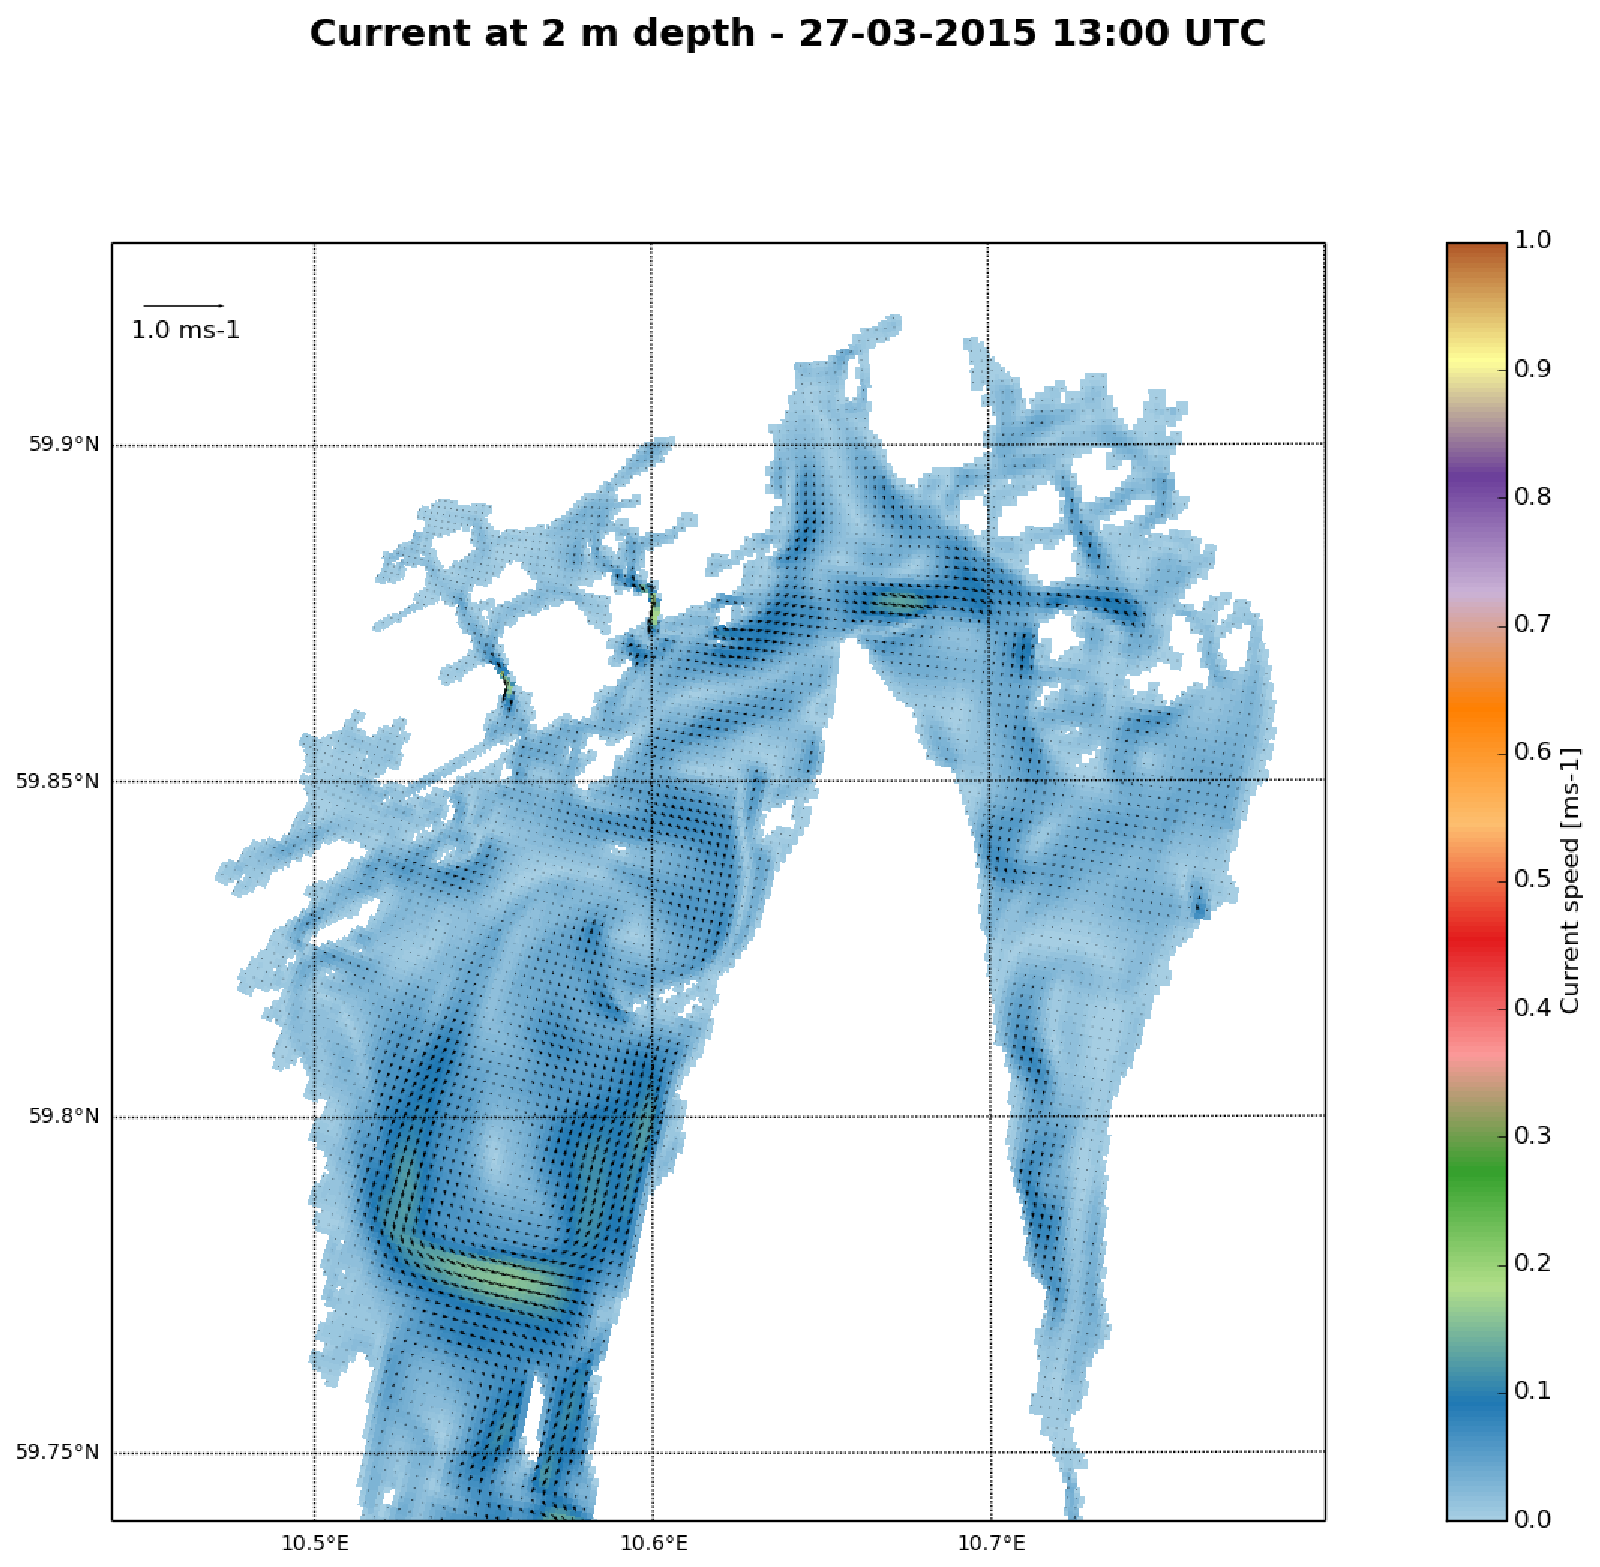
\includegraphics[height=12cm]{kap5/ferder1__0_current_crop}}
  \end{pspicture}
  \caption{\small  Currents .  }
  \label{fig:curr_oslo}
\end{figure}


 %%%%%%%%%%%%%%%%%%% Figure  %%%%%%%%%%%%%%%
\begin{figure}[t]
  \begin{pspicture}(0,0)(15,14)
% Include graphs
	\rput[b](7.5,-0.5){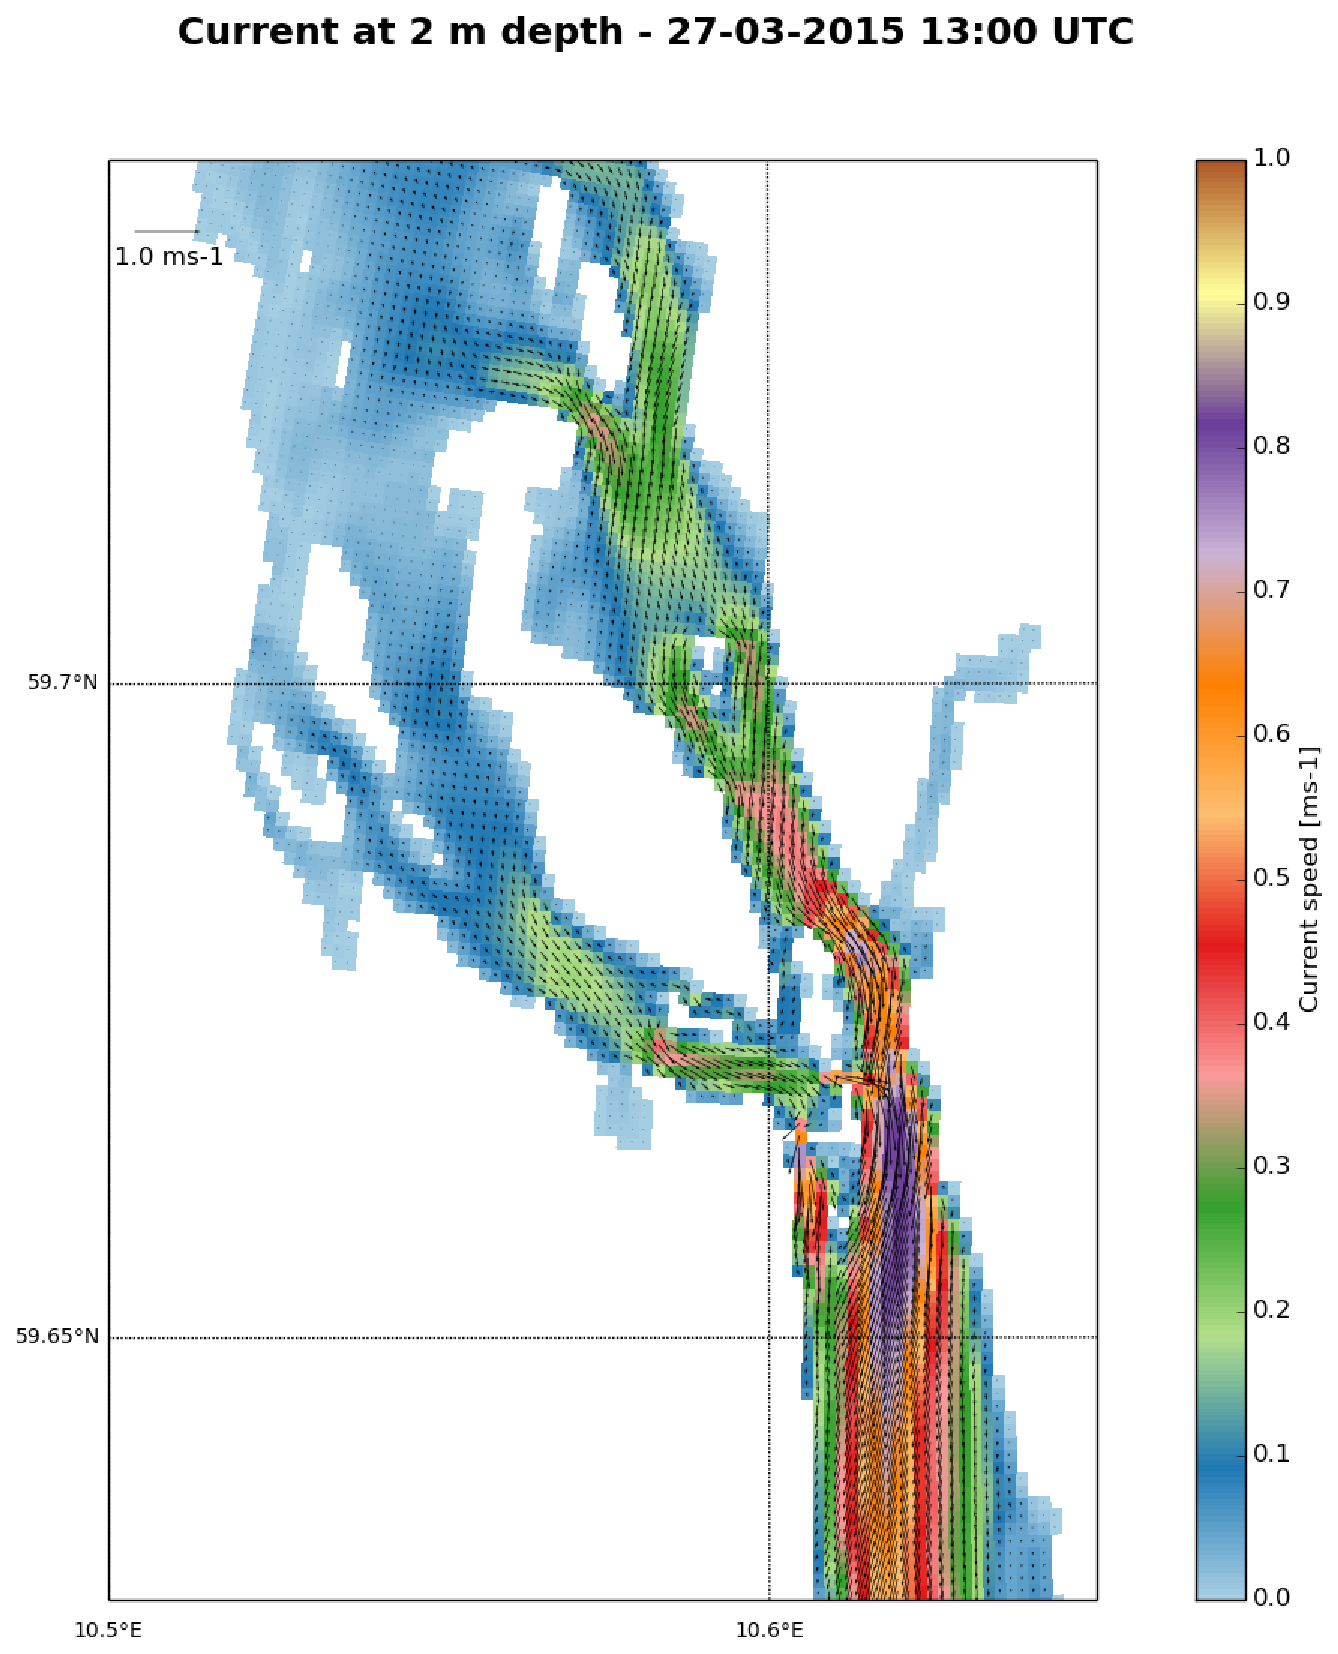
\includegraphics[height=14.5cm]{kap5/ferder2__0_current_crop}}
  \end{pspicture}
  \caption{\small As Figure \ref{fig:curr_oslo}, but for the Dr{\o}bak Sound and Vestfjorden area.}
  \label{fig:curr_drobak}
\end{figure}


 %%%%%%%%%%%%%%%%%%% Figure  %%%%%%%%%%%%%%%
\begin{figure}[t]
  \begin{pspicture}(0,0)(15,12)
% Include graphs
	\rput[b](7.5,0){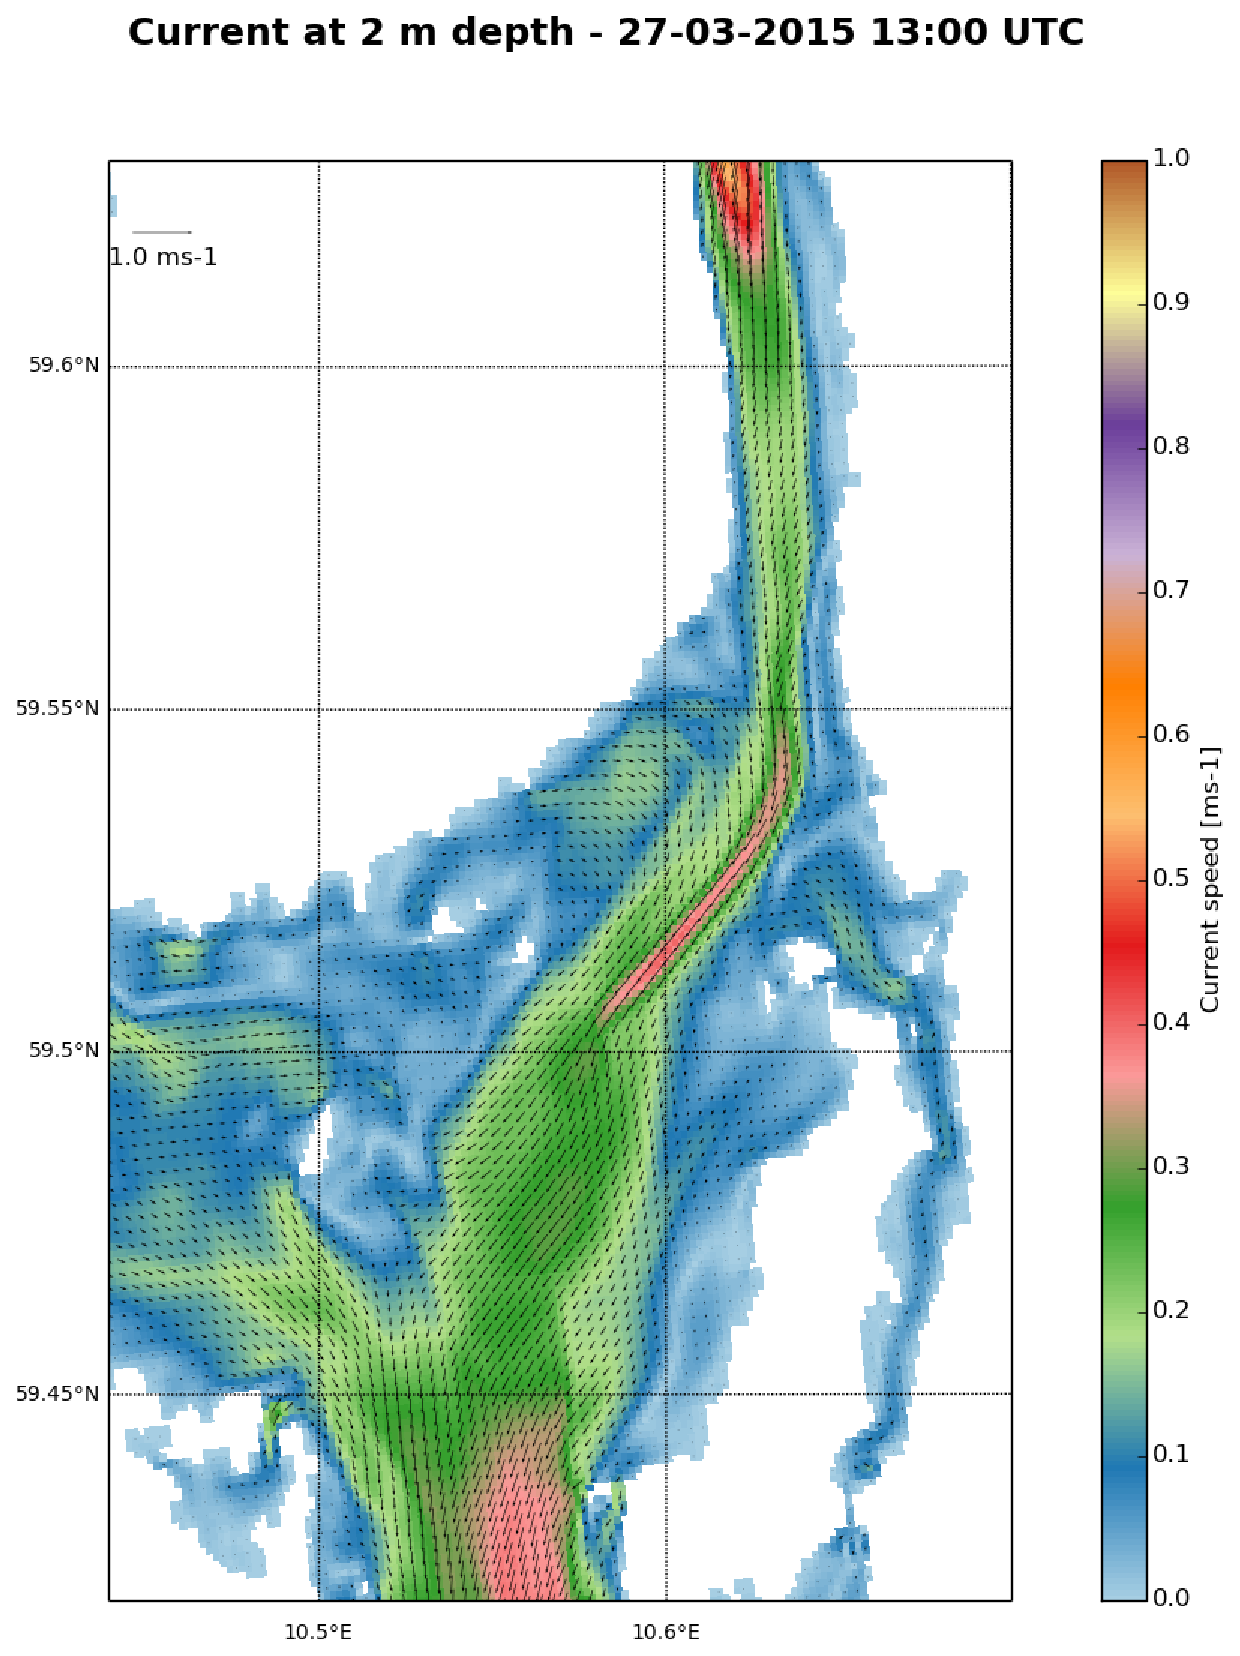
\includegraphics[height=12cm]{kap5/ferder3__0_current_crop}}
  \end{pspicture}
  \caption{\small  As for figure \ref{fig:curr_oslo}, but for the southern part of the Dr{\o}bakssund and Breidangen area.  }
  \label{fig:curr_breiangen}
\end{figure}

  

As revealed by Figure \ref{fig:curr_drobak} the speed in the {\DR} Sound is much stronger with speeds bordering on 1 m/s. We also note the presence of the Jetty obstructing the western southward flow to pass through the two narrow openings in the Jetty. The picture is one of a strong outflow in which the flow in the {\DR} Sound is a jet hugging more or less the western bank due to the effect of the Earth's rotation.   

As we proceed southwards into Breiangen the fjord widens (Figure \ref{fig:curr_breiangen}). The jet like outflow from the {\DR} Sound continues southward and is clearly guided by the topography. Nevertheless, rich details in the current patterns on its flanks  are clearly visible. As revealed also Drammenselva is discharging its water into Breiangen through the Drammensfjord. Note that the simulation replicates the swift current through the narrow opening between Drammensfjorden and Breiangen at Svelvik.  
% %%%%%%%%%%%%%%%%%%% Figure  %%%%%%%%%%%%%%%
\begin{figure}[t]
  \begin{pspicture}(0,0)(15,16)
% Include graphs
	\rput[b](7.5,0){
\includegraphics[height=16cm]{kap5/drammen1__0_current_crop}}
  \end{pspicture}
  \caption{\small  As for figure \ref{fig:curr_oslo}, but for the Drammensfjord and western Breidangen area.  }
  \label{fig:curr_drammen}
\end{figure}


 %%%%%%%%%%%%%%%%%%% Figure  %%%%%%%%%%%%%%%
\begin{figure}[t]
  \begin{pspicture}(0,0)(15,16)
% Include graphs
	\rput[b](7.5,0){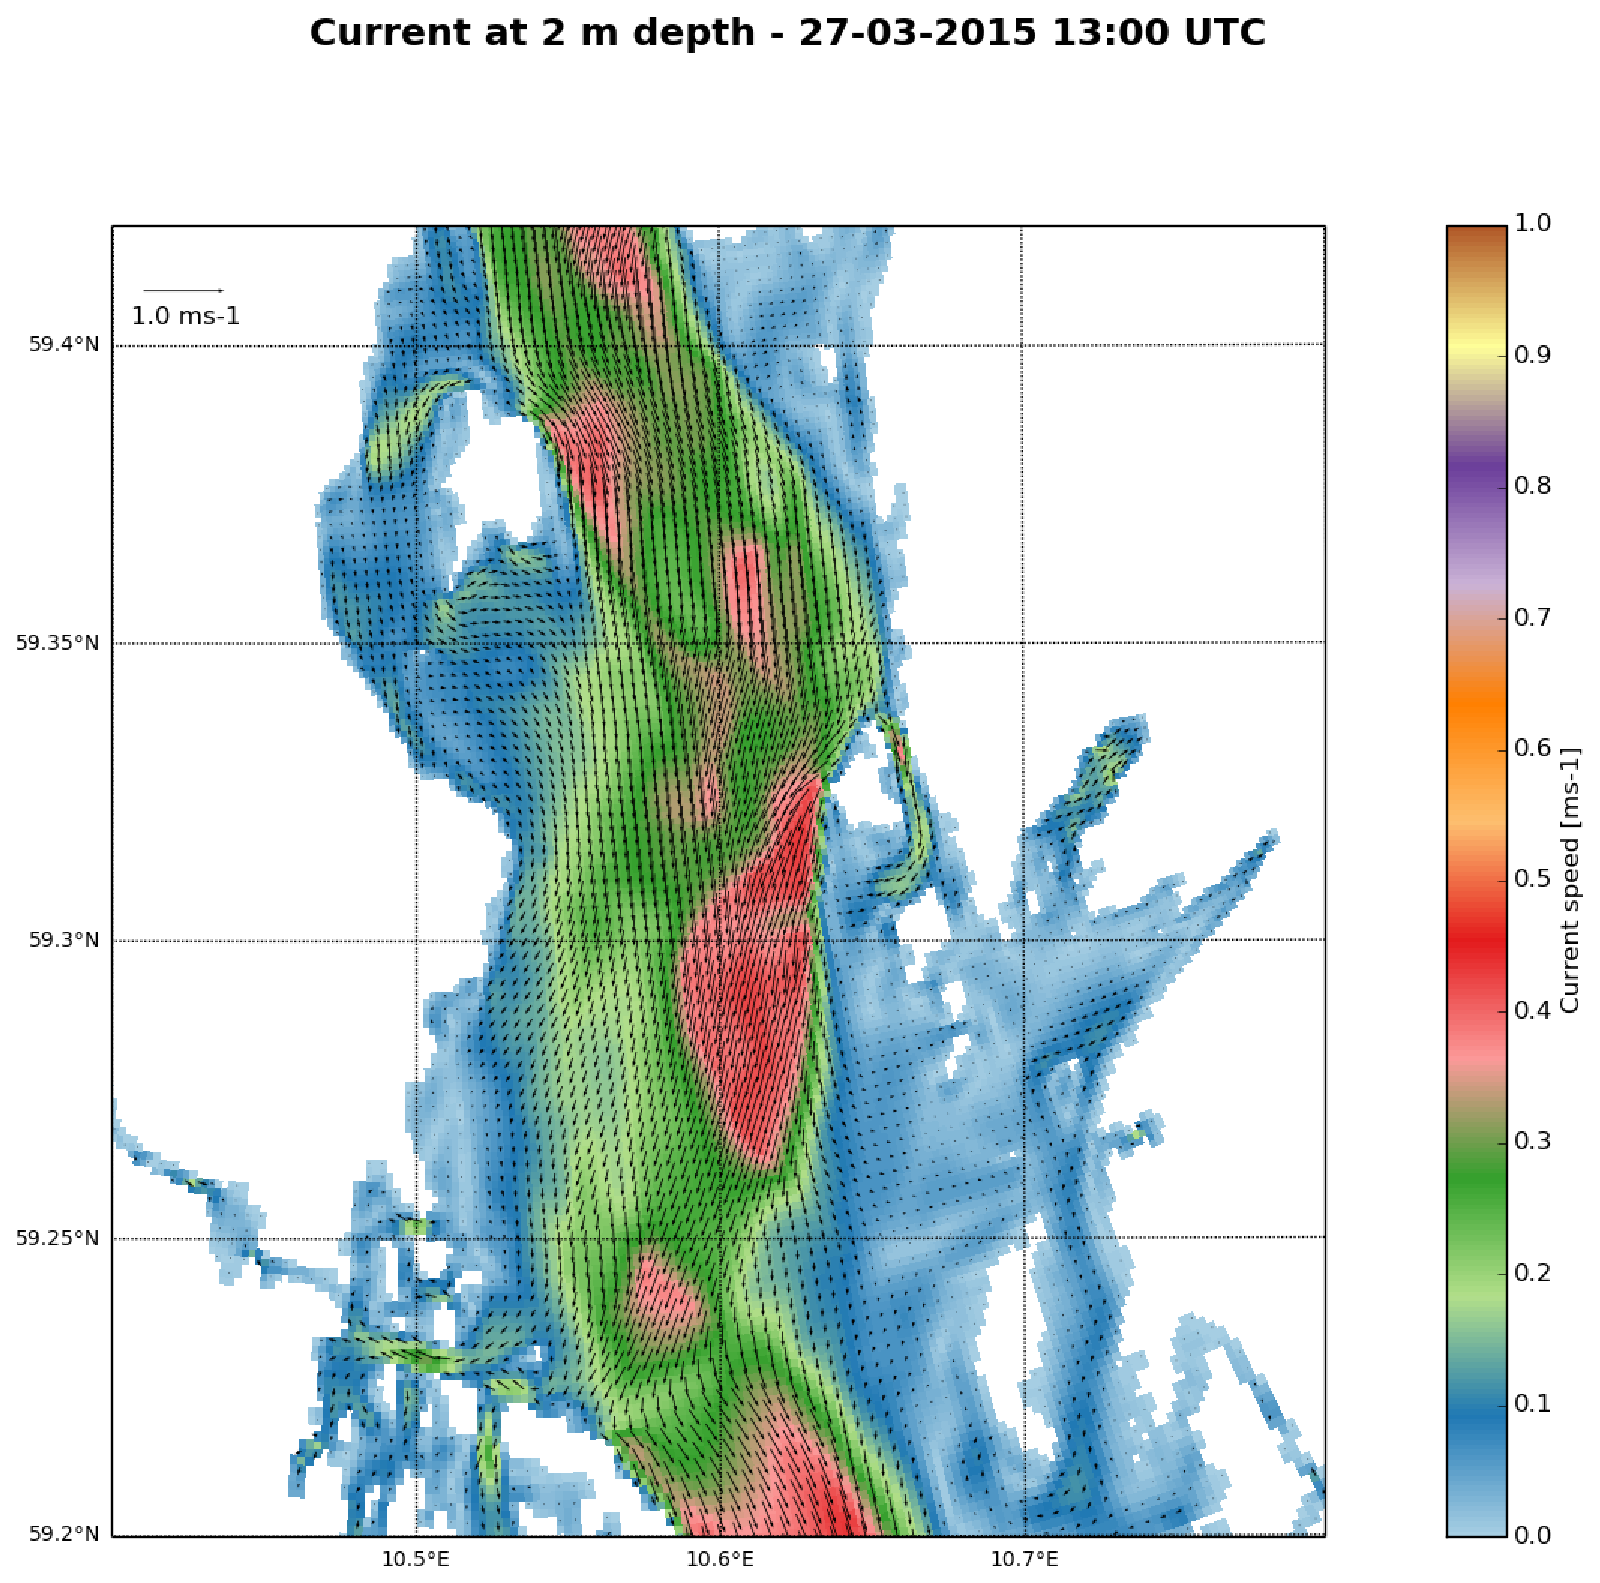
\includegraphics[height=16cm]{kap5/ferder4__0_current_crop}}
  \end{pspicture}
  \caption{\small  As Figure \ref{fig:curr_oslo}, but for the area between the Bast{\o}y, Rauer and Bol{\ae}rne islands.  }
  \label{fig:curr_mefjord}
\end{figure}



Moving further south the topography usher the jet like outflowing current to follow the deeper parts of the fjord. Hence it meanders southward toward Bol{\ae}rne (Figure \ref{fig:curr_mefjord}). Due to the strong main outflow we observe that water is forced to flow through many of the narrow sounds, straits and other openings between islands.    
 %%%%%%%%%%%%%%%%%%% Figure  %%%%%%%%%%%%%%%
\begin{figure}[t]
  \begin{pspicture}(0,0)(15,12)
% Include graphs
	\rput[b](7.5,0){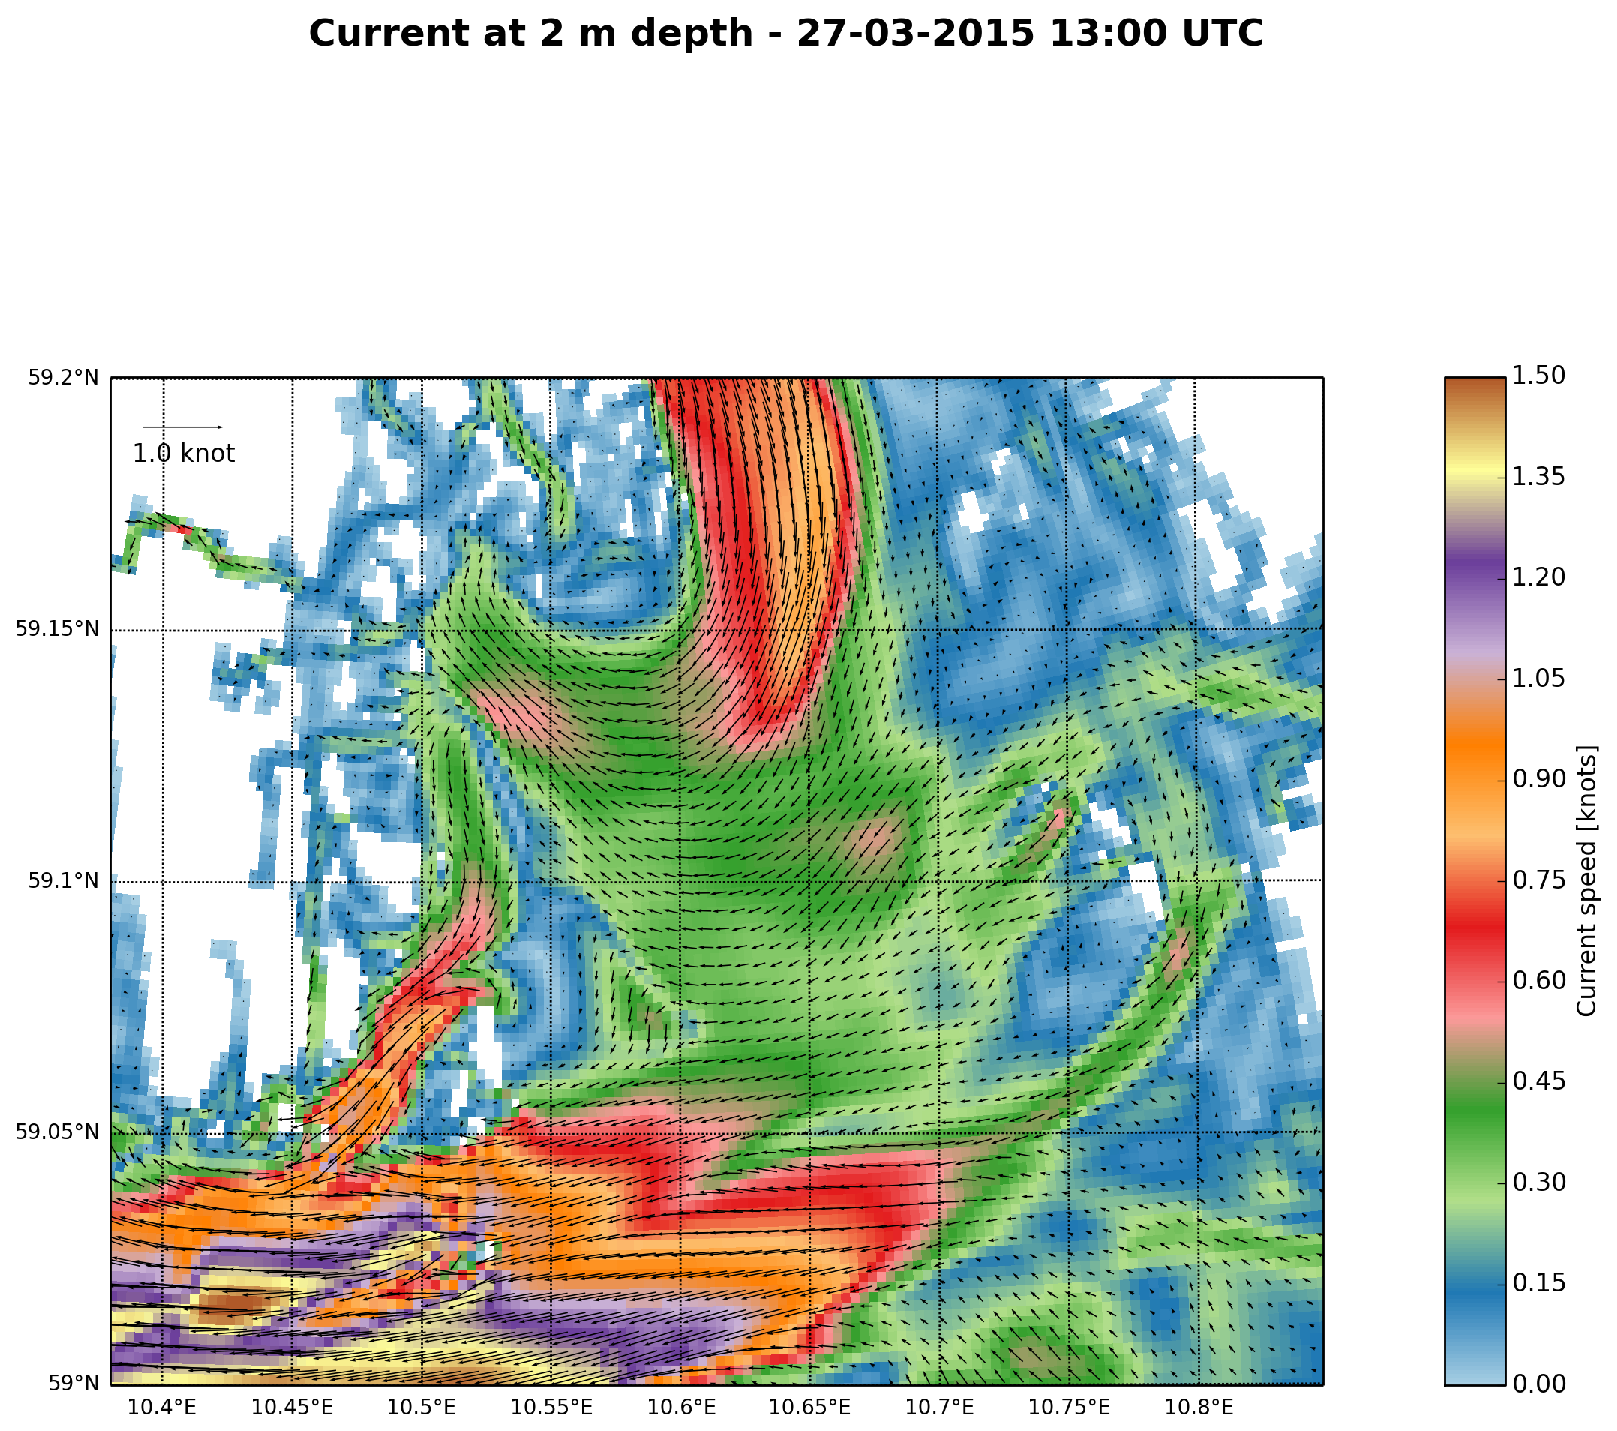
\includegraphics[height=12cm]{kap5/ferder5__0_current_crop}}
  \end{pspicture}
  \caption{\small  As for figure \ref{fig:curr_oslo}, but for the area around the F{\ae}rder lighthouse.  }
  \label{fig:curr_faerder}
\end{figure}

 

Finally the major outflow is emptied into Skagerrak as the flow is getting close to the southern border of the FjordOs CL model domain. Due to the cyclonic motion in the Skagerrak the outflowing water is guided westward and flows inside of Store F{\ae}rder to join the westward flowing current in the Skagerrak.    

In summary the circulation pattern in upper water masses in the Oslofjord on March 23, 2015 is one of strong outflow that more or less is guided by the topography and hence meanders as it flows southward. In addition to this general flow the circulation pattern reveals detailed currents flowing through the many straits, narrow sounds and opening between islands. The latter is only made possible by the high resolution offered by the new FjordOs CL model.

\clearpage
\subsection{Hydrography and sea level}
\label{subsec:hydro}
It is also interesting to note the rich detail in the salinity and temperature patterns only made possible due to the high resolution of FjordOs CL model as revealed by Figures \ref{fig:salt_hele} and \ref{fig:temp_hele}). Nevertheless the most striking feature to be observed is the impact of the rivers. In particular this is evident looking at the salinity distribution (Figure \ref{fig:salt_hele}). In March the river discharge is starting to peak and hence increasing the freshwater content in the upper water masses of the fjord and in particular close to their mouths. This is particularly evident for the two major rivers Glomma and Drammenselva, but also clearly visible regarding Numedalsl{\aa}gen and Aulivassdraget (T{\o}nsberg). At these locations the temperature is somewhat increased, in particular in the Drammensfjord, in comparison to the rest of the fjord. We believe this is due to entrainment of warm water from below due to the swift currents created there.

Regarding the water level at March 23, 2015 (Figure \ref{fig:ssh_hele}) we observe that this date is one of high sea level in the inner parts with lower sea levels as we proceed southwards. This is in line with the strong outflow described in Section \ref{subsec:curre} above.
 %%%%%%%%%%%%%%%%%%% Figure  %%%%%%%%%%%%%%%
\begin{figure}[t]
  \begin{pspicture}(0,0)(15,12)
% Include graphs
	\rput[b](7.5,0){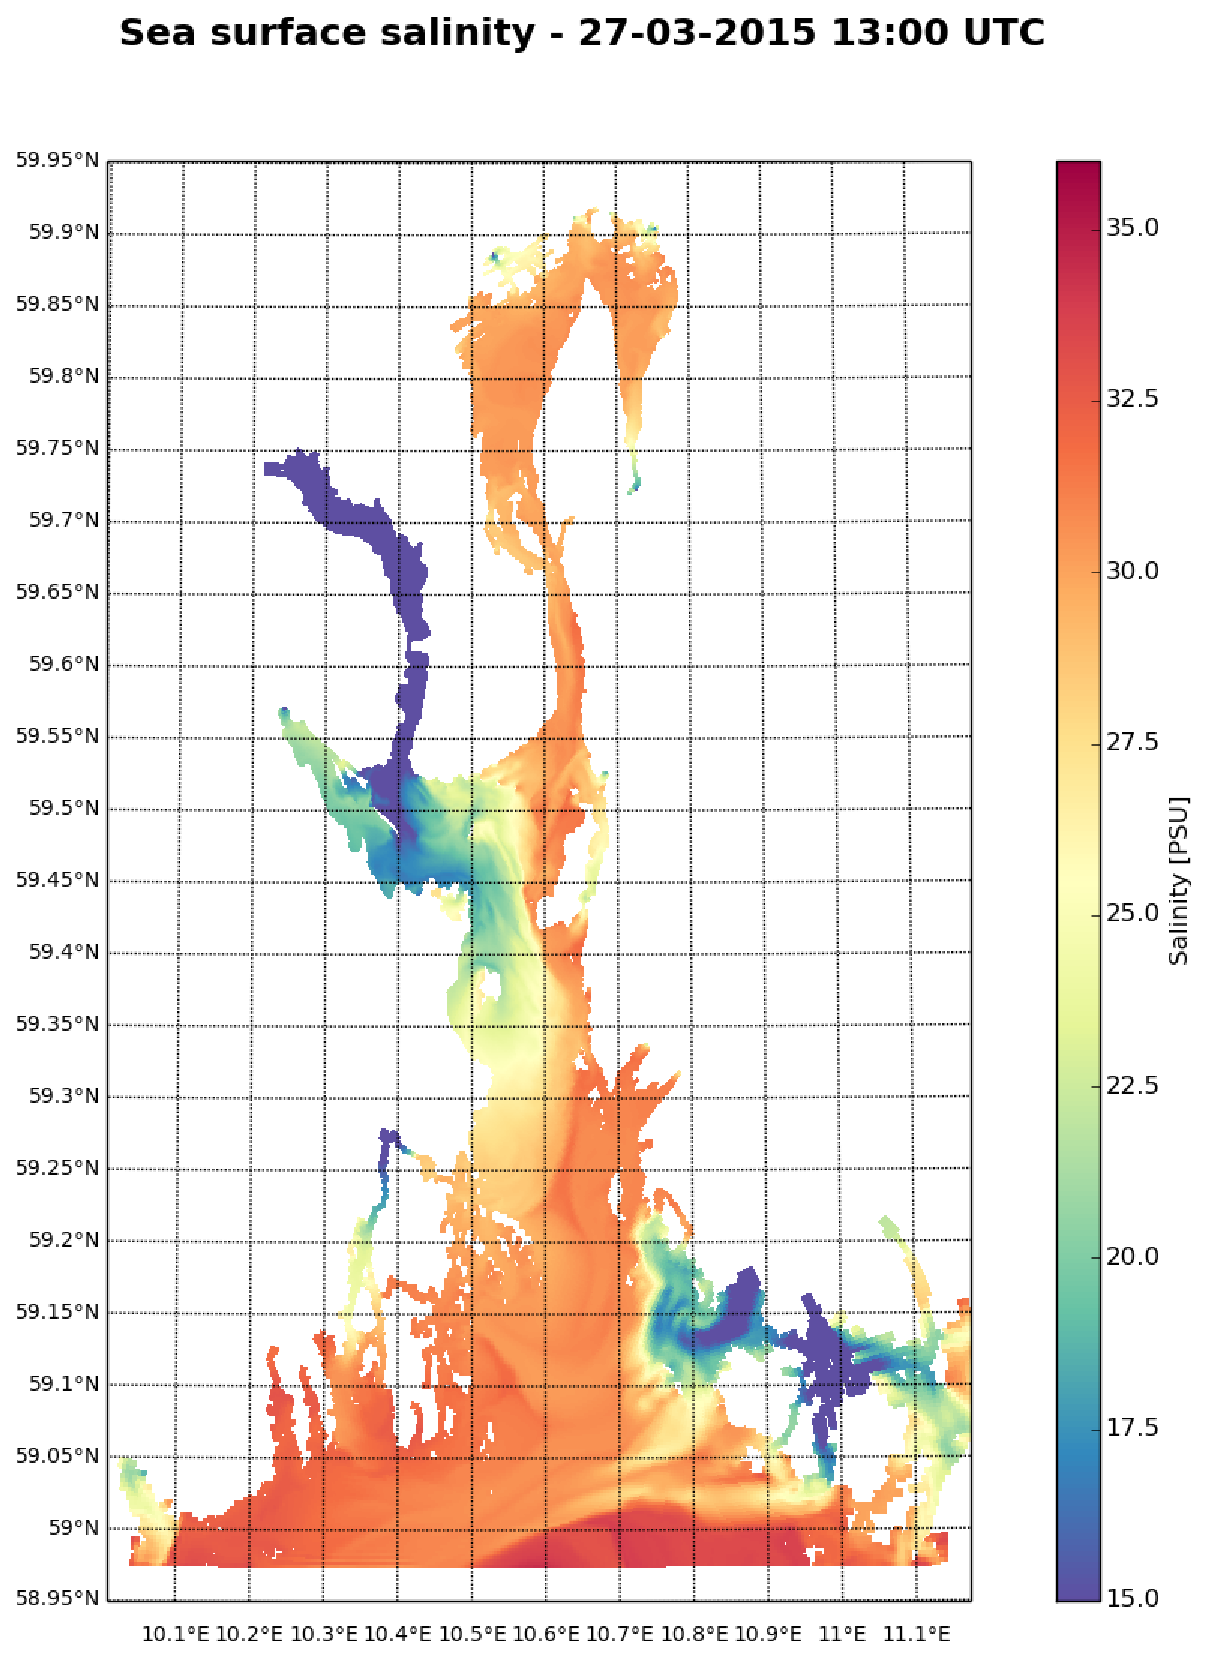
\includegraphics[height=12cm]{kap5/salt_hele_0_current_crop}}
  \end{pspicture}
  \caption{\small  As for figure \ref{fig:temp_hele}, but for sea surface salinity (SSS).  }
  \label{fig:salt_hele}
\end{figure}

  
 %%%%%%%%%%%%%%%%%%% Figure  %%%%%%%%%%%%%%%
\begin{figure}[t]
  \begin{pspicture}(0,0)(15,12)
% Include graphs
	\rput[b](7.5,0){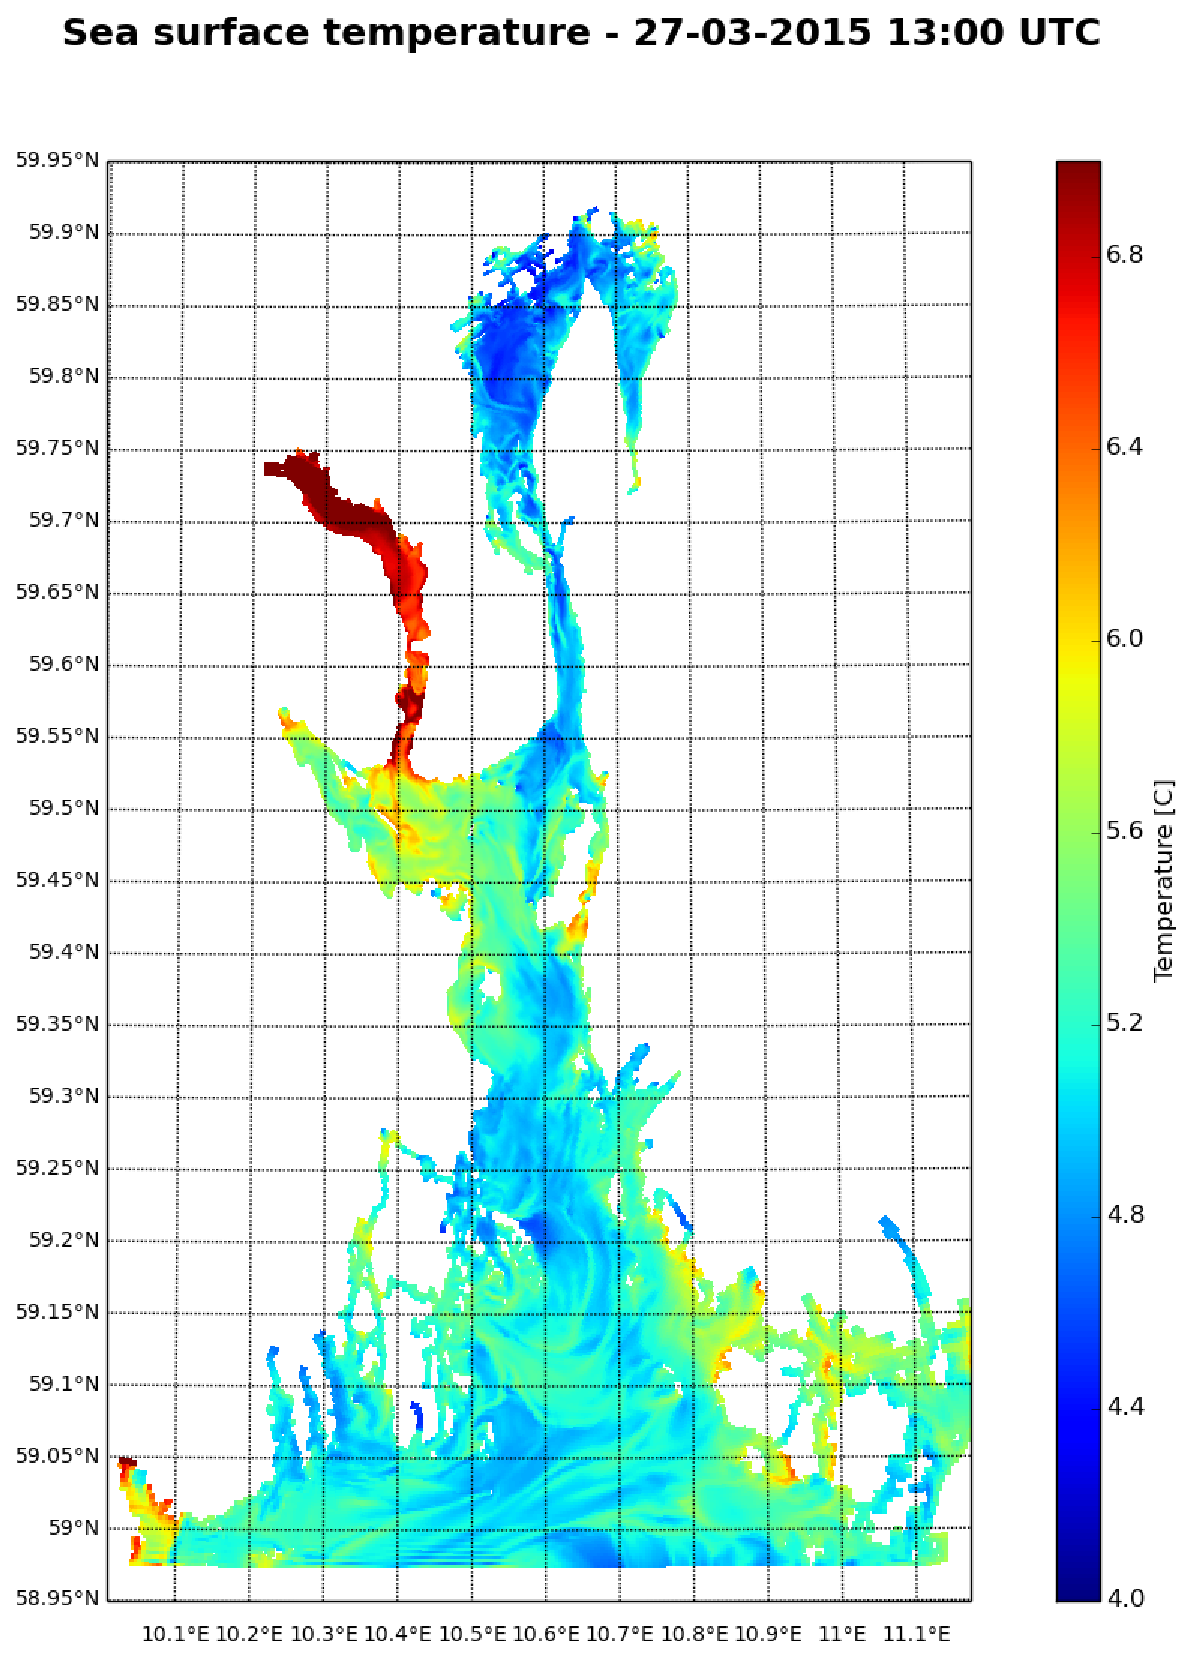
\includegraphics[height=12cm]{kap5/temp_hele_0_current_crop}}
  \end{pspicture}
  \caption{\small  Sea surface temperature (SST) for the entire model domain of the FjordOs model. Note the high SST in the Drammensfjorden area. We believe this is not realistic, and is most likely cause by the mixing up of warmer water from below. This warm water is probably left from imperfect initial conditions. }
  \label{fig:temp_hele}
\end{figure}

 
 %%%%%%%%%%%%%%%%%%% Figure  %%%%%%%%%%%%%%%
\begin{figure}[t]
  \begin{pspicture}(0,0)(15,17)
% Include graphs
	\rput[b](7.5,0){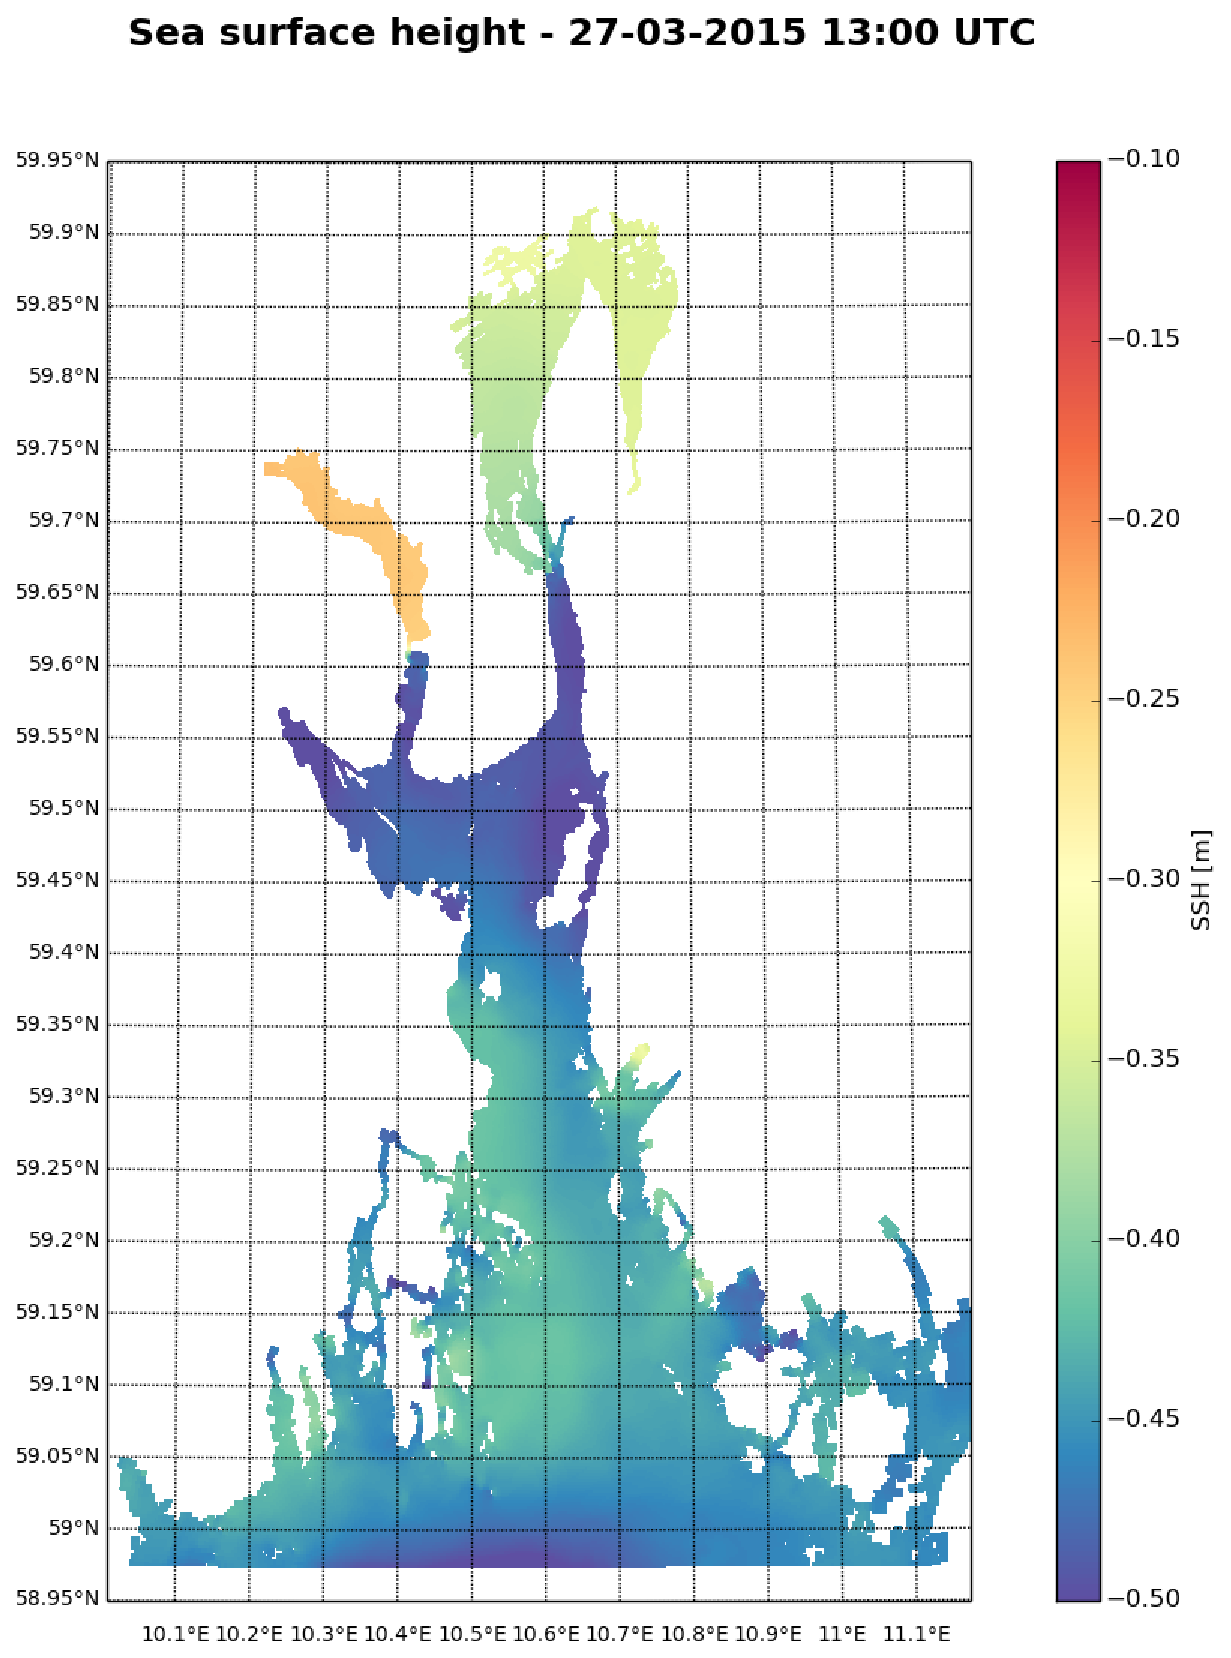
\includegraphics[height=17cm]{kap5/zeta_hele_0_crop}}
  \end{pspicture}
  \caption{\small  As for figure \ref{fig:temp_hele}, but for sea surface height (SSH).  }
  \label{fig:ssh_hele}
\end{figure}

  
\clearpage
